\section{Zielsetzung}
In diesem Versuch soll der Brechungsindex $n$ anhand der Intensität reflektierten und gebrochenen Lichts untersucht werden.\\ 


\section{Theorie}
\label{sec:Theorie}

\subsection{Poynting-Vektor}
Aus den Maxwell-Gleichungen lässt sich schlussfolgern, dass die 
Strahlungsintensität je Flächeneinheit durch den Poynting-Vektor
\begin{equation*}
    |\vec{S}| = v \cdot \varepsilon_0 \cdot \varepsilon \cdot \vec{E}^2
\end{equation*}
beschreiben lässt.
Hier ist $\vec{S}$ der Poynting-Vektor, $\vec{E}$ das elektrische Feld, der Dielektrizitätskonstante $\varepsilon$ und der 
elektrischen Feldkonstante $\varepsilon_0$.\\
Es ergibt sich so die Beziehung
\begin{equation*}
\mathrm{n}^2 = \varepsilon
\end{equation*}
zwischen Brechungsindex $n$ und Dielektrizitätskonstante $\varepsilon$.\\



 \subsection{Verhalten an Grenzflächen}
Bein Einfall einer ebenen Welle im Vakuum unter dem Winkel $\alpha$ auf eine Grenzfläche 
wird ein Teil reflektiert, der andere transmittiert in das Medium. \\
Für die Amplituden verhält es sich entsprechend.\\
Da die Ausbreitungsgeschwindigkeit sich im Medium ändert (kleiner wird), wird, wie in \autoref{fig:brechung} zu sehen,  die 
Richtung des Strahls geändert und der Brechungswinkel $\beta < \alpha$ tritt auf.\\
\begin{figure} [H]
    \centering
    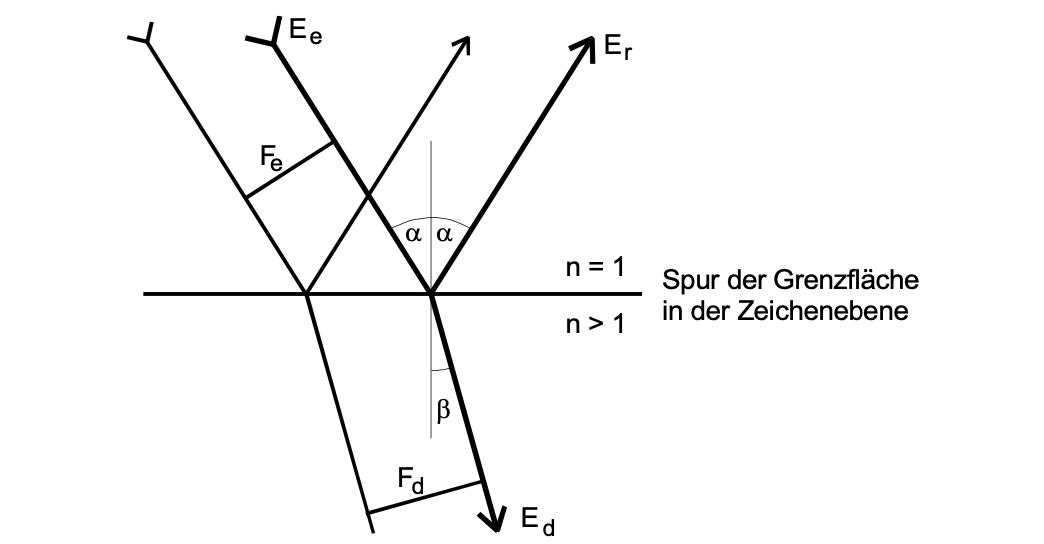
\includegraphics{content/brechung}
    \caption{Das Verhalten einer aus dem Vakuum in eine Grenzfläche einfallenden Welle. \cite{sample}}
    \label{fig:brechung}
  \end{figure}
Aus der Energieerhaltung folgt 
\begin{equation*}
    (\vec{E_e}^2 - \vec{E_r}^2)  \cdot cos(\alpha) =  \mathrm{n} \cdot \vec{E_d}^2 \cdot cos(\beta),
\end{equation*}
sodass in konkreteren Berechnungen zwischen senkrechter und paralleler Polarisationsrichtung 
unterschieden werden muss.
Die Polarisationsrichtung wird relativ zur Einfallsebene gemessen, welche durch den einfallenden 
und reflektierten Strahl aufgespannt wird. \\ 


\subsection{Senkrecht polarisiertes Licht}
Bei senkrecht polarisiertem Licht schwingt der $\vec{E_\bot}$ Vektor tangential zur Grenzfläche.\\
Da ein Linienintegral von $\vec{E}$ über eine geschlossene Kurve sich zu Null ergibt, lässt sich schlussfolgern, dass 
die tangentiale Komponente die Grenzfläche stetig passiert.\\›
Durch die Stetigkeit bedingt gilt
\begin{equation*}
    \vec{E_r}_\bot = -\vec{E_e}_\bot \cdot \frac{n cos(\beta)-cos(\alpha)}{n cos(\beta)+cos(\alpha)}
\end{equation*}
und mit Hilfe des Snelliusschen Brechungsgesetzes $n = \frac{sin(\alpha)}{sin(\beta)}$ folgt 
\begin{equation*}
    \vec{E_r}_\bot = -\vec{E_e}_\bot \cdot \frac{(\sqrt{\mathrm{n^2} - sin^2(\alpha)} - cos(\alpha))^2}{n^2 - 1}
\end{equation*}

 \subsection{Parallel polarisiertes Licht}
Bei senkrecht polarisiertem Licht schwingt der $\vec{E_\bot}$ Vektor in zur Einfallsebene.\\
Analog zur senkrechten Polarisation folgt hier
\begin{equation*}
    \vec{E_r}_\shortparallel  = \vec{E_e}_\shortparallel  \cdot \frac{n cos(\alpha)-cos(\beta)}{n cos(\alpha)+cos(\beta)}
\end{equation*}
aus der Stetigkeitsbedingung.\\
Mit Snellius ergibt sich  
\begin{equation*}
    \vec{E_r}_\shortparallel  = \vec{E_e}_\shortparallel  \cdot \frac{n^2 cos(\alpha) - \sqrt{\mathrm{n^2} - sin^2(\alpha)}}{n^2 cos(\alpha) - \sqrt{\mathrm{n^2} + sin^2(\alpha)}}
\end{equation*}
für die Winkelabhängigkeit.\\
Im Falle $\alpha + \beta = 90°$ verschwindet die reflektierte Komponente des parallel polarisierten Lichts. Der Strahl tritt also
vollständig in das Medium ein.\\
Nach Snellius lässt sich die Gleichung für den Brechungsindex zu 
\begin{equation*}
    n = tan(\alpha)
\end{equation*}
vereinfachen. \\

